% !TEX program = xelatex
%% Requires compilation with XeLaTeX or LuaLaTeX
\documentclass[10pt,xcolor={table,dvipsnames},t]{beamer}
\usepackage{biblatex}
\usepackage{caption}
\setbeamertemplate{caption}[numbered]
\addbibresource{reference.bib}
\usepackage{hyperref}
\hypersetup{ 
pdfpagemode=FullScreen,  
colorlinks=true,linkcolor=blue}
\usepackage{enumerate}

\usepackage{listings}
\usepackage{xcolor}

\definecolor{codegreen}{rgb}{0,0.6,0}
\definecolor{codegray}{rgb}{0.5,0.5,0.5}
\definecolor{codepurple}{rgb}{0.58,0,0.82}
\definecolor{backcolour}{rgb}{0.95,0.95,0.92}

\lstdefinestyle{mystyle}{
    backgroundcolor=\color{backcolour},   
    commentstyle=\color{codegreen},
    keywordstyle=\color{magenta},
    numberstyle=\tiny\color{codegray},
    stringstyle=\color{codepurple},
    basicstyle=\ttfamily\footnotesize,
    breakatwhitespace=false,         
    breaklines=true,                 
    captionpos=b,                    
    keepspaces=true,                 
    numbers=left,                    
    numbersep=5pt,                  
    showspaces=false,                
    showstringspaces=false,
    showtabs=false,                  
    tabsize=2
}

\lstset{style=mystyle}

% Flow chart config
\usepackage{tikz}
\usetikzlibrary{calc,trees,positioning,arrows,fit,shapes,calc}
\usetikzlibrary{shapes.geometric, arrows}
\tikzstyle{startstop} = [rectangle, rounded corners, minimum width=3cm, minimum height=1cm,text centered, draw=black, fill=red!30]
\tikzstyle{io} = [trapezium, trapezium left angle=70, trapezium right angle=110, minimum width=3cm, minimum height=1cm, text centered, draw=black, fill=blue!30]
\tikzstyle{process} = [rectangle, minimum width=3cm, minimum height=1cm, text centered, draw=black, fill=orange!30]
\tikzstyle{decision} = [diamond, minimum width=3cm, minimum height=1cm, text centered, draw=black, fill=green!30]
\tikzstyle{arrow} = [thick,->,>=stealth]

\usetheme{UCBerkeley}

\title[Your Short Title]{STMC HKOI Training}
\subtitle{Mathematical Foundations}
\author{Chan Yan Mong}
%\institute{}
\date{\today}

\begin{document}

\begin{frame}
  \titlepage
\end{frame}

% Uncomment these lines for an automatically generated outline.
%\begin{frame}{Outline}
%  \tableofcontents
%\end{frame}

\section{Elementary Knowledge}
\subsection{Exponent}
\begin{frame}{Exponent Notation}
    \begin{itemize}
      \item Many times in mathematics we encounter expressions that involve repeated multiplications of same number
      \item E.g. $2\times 2 \times 2 \times 2; \quad \overbrace{4\times 4\cdots \times 4}^{51 \, \text{times}}$
      \item To simply our notation, we will introduce the \textbf{exponent notation}
    \end{itemize}
\end{frame}

\begin{frame}{Exponent Notation}
  \begin{definition}[Positive Exponent]
    Let $N\in \mathbb{Z}^{+}$ and $m\in \mathbb{R}$. The $N$ th power of $m$, denoted $m^N$, is defined as:
    \begin{equation}
      m^N = \overbrace{m \times m \times \cdots \times m \times m}^{N\,\text{times}}
    \end{equation}
    For example, in previous examples:\\
     $2\times 2 \times 2 \times 2 = 2^4$ and $\quad$ $\overbrace{4\times 4\cdots \times 4}^{51 \, \text{times}} = 4^{51}$
  \end{definition}
\end{frame}

\begin{frame}{Properties of exponent}
  It's easy to proof that the exponent satisfy the following properites:
  \begin{theorem}[Properties of exponent]
    \begin{enumerate}
      \item $a^m a^n = a^{m+n} \quad m,n\in \mathbb{Z}^+$
      \item $a^m/a^n = a^{m-n} \quad m,n \in \mathbb{Z}^+, m>n$
      \item $(a^m)^n = a^{mn} \quad m,n \in \mathbb{Z}^+$
    \end{enumerate}
    \begin{proof}
      Omitted, explain in class
    \end{proof}
  \end{theorem}
\end{frame}

\begin{frame}{Extending exponent}
  \begin{itemize}
    \item To make the theorems above more useful, we define extend our definition of exponent in the following way:
  \end{itemize}
  \begin{definition}[Negative and Zero exponent]
    Let $N\in \mathbb{Z}$ and $m\in \mathbb{R}$. The $N$ th power of $m$, denoted $m^N$, is defined as:
    \begin{equation}
      m^N = \begin{cases}
        \overbrace{m \times m \times \cdots \times m \times m}^{N\,\text{times}},& N > 0 \\
        1, & N = 0\\
        1/m^{|N|},&N <0

      \end{cases}
    \end{equation}
  \end{definition}
\end{frame}

\begin{frame}{Extending exponent}
  Examples:
  \begin{itemize}
    \item $2^0 = 1$
    \item $6^{-3} = 1/6^3$
  \end{itemize}
  Such notation is very useful. Consider the following expression:
  \begin{align*}
    S &= \frac{1}{2} + \frac{1}{6} + \frac{1}{16}\\
    &= 2^{-1} + \left(2^{-1}\right)\left(3^{-1}\right) + 2^{-4}\\
    &= \left(2^{-4}\right)\left(3^{-1}\right) \left[ \left(2^3\right)\left(3^1\right) + 2^3 + 3^1\right]\\
    &= \frac{35}{48}
  \end{align*}
\end{frame}

\begin{frame}{Fractional exponent}
  \begin{itemize}
    \item In a similar vein, we can define fractional exponent using the multiplication rule:
    \begin{align*}
      \left(m^{1/N}\right)^N = m^{N/N} = m
    \end{align*}
    Hence:
    \begin{equation*}
      m^{1/N} = \sqrt[N]{m}
    \end{equation*}
  \end{itemize}
\end{frame}

\begin{frame}{Fractional exponent}
  \begin{definition}[Fractional exponent]
    Let $m \in \mathbb{R}$ and $m>0$ and $N\in \mathbb{Z}$, then we define the fractional exponent of $m$ as:
    \begin{equation}
      m^{1/N} = \sqrt[N]{m}
    \end{equation}
    where $\sqrt[N]{\cdots}$ denotes the $N$-th root of the number
  \end{definition}
\end{frame}

\begin{frame}{Loop: Repeat and repeat ....}
  \begin{itemize}
    \item From the examples above, we see the a looping structure always consist of two parts:
    \begin{enumerate}
      \item The code inside the code that is looped over 
      \item A condition that is checked everytime the loop ran to decide whether the loop should continue
    \end{enumerate}
    \item  Example: 
    \begin{itemize}
      \item Recieving user input (code inside loop); Is the answer right (terminate condition)
      \item Reading files (code inside loop); Is the end of file reached (terminate condition)
      \item Main game code (code inside the loop); Is the game over (terminate condition)
      \item Searching for answers (code inside the loop); Is the solution found (terminate condition)
    \end{itemize}
  \end{itemize}
\end{frame}

\begin{frame}{Types of loop}
  \begin{itemize}
    \item Loops can also be classified into two categories:
    \begin{enumerate}
      \item \textbf{Pre-check loops} and
      \item \textbf{Post-check loops}
    \end{enumerate}
    \item In this lesson we will focus on post-check loops and deal with pre-check loops next lesson
  \end{itemize}
\end{frame}

\begin{frame}[fragile]{\texttt{while} loop}
  \begin{exampleblock}{Example: Print first $N$ positive integers}
    \begin{itemize}
      \item Suppose you want to write a program that takes in an integer $N$ and print out all positive integers $\leq N$. We can implement that using while loop.
      \item For example:
\begin{lstlisting}
  $./main       $./main       $./main 
  5             4             100
  1             1             1
  2             2             2
  3             3             .... /* too long won't list here*/
  4             4             99
  5                           100
\end{lstlisting}
    \end{itemize}
  \end{exampleblock}
\end{frame}

\begin{frame}{\texttt{while} loop}
  \begin{columns}
    \column{0.6\textwidth}
    \begin{itemize}
      \item Let's look at the flowchart of the program
      \item Here the looping condition is $i \leq N$ and the main code that is looped is "Print i" and "Set i = i + 1"
      \item Notice "Set i = i + 1" is crucial otherwise i will always be smaller than N. This will cause an \textbf{infinite loop}
    \end{itemize}
    \column{0.4\textwidth}
    \begin{figure}
      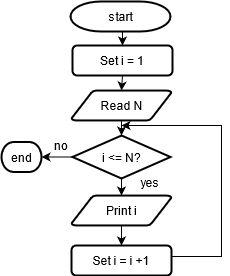
\includegraphics[width=0.9\textwidth]{img/print_first_n_flowchart.png}
    \end{figure}
  \end{columns}
\end{frame}

\begin{frame}[fragile]{\texttt{while} loop}
  \begin{itemize}
    \item Let's implement the code in C/C++
    \item Notice when the condition is \texttt{true}, it will loop
  \end{itemize}
\begin{lstlisting}[language=C]
int i = 1, N;
scanf("%d",&N);

/* The while loop */
while(i <= N) {     // Is i <= N? If true then loop
  printf("%d\n",i); // Print i 
  i = i + 1;        // Set i = i + 1
}
\end{lstlisting}
\end{frame}

\begin{frame}{\texttt{while} loop}
  \begin{exampleblock}{Example: Sum of first $n$ cubes}
    Write a program that takes $n$ as an input and compute the sum of first $n$ cubes $S_n$:
    \begin{align*}
      S_1 &= 1^3\\
      S_2 &= 1 + 2^3\\
      \cdots \\ 
      S_n &= 1^3 + 2^3 + \cdots  + (n-1)^3 + n^3
    \end{align*}
  \end{exampleblock}
\end{frame}

\begin{frame}[fragile]{\texttt{while} loop}
  \begin{itemize}
    \item This is similar to our previous example:
  \end{itemize}
\begin{lstlisting}[language=C]
int i = 1, sum = 0, N;
scanf("%d",&N);

/* The while loop */
while(i <= N) {     // Is i <= N? If true then loop
  sum = sum + i*i*i;
  i = i + 1;
}

printf("Required sum: %d\n",sum);
\end{lstlisting}
\end{frame}

\begin{frame}[fragile]{\texttt{while} loop}
  \begin{exampleblock}{Example: Input validation}
    \begin{itemize}
      \item Suppose we are writing a program that computes the BMI of a student given weight and height as input using the formula $\text{BMI} = \text{weight}/\text{height}^2$
      \item Naturally, we will do something similar to this to get the input:
\begin{lstlisting}[language=C]
float height, weight;
scanf("%f %f",&height,&weight);
\end{lstlisting}
    \end{itemize}
  \end{exampleblock}
\end{frame}

\begin{frame}[fragile]{\texttt{while} loop}
    \begin{itemize}
      \item Although we know that weight and height must be larger than zero and they both have an upper bound. There are nothing stopping the user from entering the following in the program:
\begin{lstlisting}[language=bash]
./main
-100 1000000 /* People with -100m and 1000000kg ???? */
\end{lstlisting}
    \item Therefore, we need a way to check and prevent these things from happening
    \item Write a program that check if $0\leq \text{weight} \leq 600$kg and $0 \leq \text{height} \leq 3$m and keep asking the user to reenter weight and height until the correct value is recieved.
    \end{itemize}
\end{frame}

\begin{frame}[fragile]{\texttt{while} loop}
  \begin{itemize}
    \item Here is the code:
  \end{itemize}
\begin{lstlisting}[language=C]
float height, weight;
printf("Please enter height and weight: ");
scanf("%f %f",&height, &weight);

while(!(0.0 <= weight && weight <= 600.0 && 0.0 <= height && height <= 3.0)) {
  printf("Height must be between 0 to 3.0 and weight must be between 0 to 600.0!\n");
  printf("Re-enter height and weight: ");
  scanf("%f %f",&height,&weight);
}

printf("Height, weight and BMI = %f, %f, %f\n",height,weight,height/(weight*weight));
\end{lstlisting}
\end{frame}


\begin{frame}{\texttt{while} loop}
  \begin{exampleblock}{Examples: Fixed point iteration}
    \begin{itemize}
      \item Let $x,a$ be two non negative real numbers. If $x^2 = a$, then $x$ is called the square root of $a$ and we denote $x = \sqrt{a}$
      \item For example, $3^2 = 9$ so $3$ is the square root of $9$. We also denote $3 = \sqrt{9}$
      \item Now, how can we find interesting 
    \end{itemize}
  \end{exampleblock}
\end{frame}

\begin{frame}[fragile]{\texttt{if-else} statement}
  \begin{itemize}
    \item This can be done by the \texttt{if-else} statement in C/C++
    \item We ignore the \texttt{main()} part and focus on the if statement itself
  \end{itemize}
  \begin{lstlisting}[language=C]
    /* This is inside main(); I am just lazy */

    if(/* Is it raning? */){ 
      /* Stay at home */
    } else {
      /* Go out */
    }
  \end{lstlisting}
\end{frame}

\section{Comparison operators}
\begin{frame}{Filling the condition}
  \begin{itemize}
    \item But how do we fill in the \texttt{/* Is it raining ? */} part?
    \item In general, we fill that part with an \textbf{boolean expression} that return \textit{true} or \textit{false} upon evaluation
    \item For example of boolean expressions are:
    \begin{itemize}
      \item Is x > y ?
      \item Is x equal to y?
      \item etc.
    \end{itemize}
    \item Let's look at some examples to see how exactly can we do that in C/C++
  \end{itemize}
\end{frame}

\section{Comparison operators}
\begin{frame}{Equal to \texttt{==}}
  \begin{itemize}
    \item The operator \texttt{==} is the operator for \textbf{equal to}
    \item \textbf{Do not confuse it with a single =}
    \item \texttt{x==y} checks if x is equal to y
    \item An example of the so called \textit{comparsion operators}
    \item Examples:
    \begin{itemize}
      \item \texttt{1 == 0} $\rightarrow$ \texttt{false}
      \item \texttt{3 == 3} $\rightarrow$ \texttt{true}
      \item \texttt{'a' == 'A'} $\rightarrow$ \texttt{false}
      \item \texttt{'b' == 'b'} $\rightarrow$ \texttt{true}
    \end{itemize}
  \end{itemize}
\end{frame}
\begin{frame}{Equal to \texttt{==}}
  \begin{exampleblock}{Example:}
    John is a middle schooler. Everyday he can either be happy or unhappy. If he is happy, he will study; If he is not, he will play computer games. Let \texttt{happiness} be John's happiness. If \texttt{happiness} is 1, he is happy; otherwise, he is not. Write a program that predicts what John will do given his happiness.
  \end{exampleblock}
  \vspace{1mm}
  \textbf{Input:} An integer \texttt{happiness} which is either 0 or 1\\
  \textbf{Output:} Print "He will study" if he is happy and "He will play computer games" if not.
\end{frame}

\begin{frame}[fragile]{Equal to \texttt{==}}
\begin{lstlisting}[language=C]
#include <stdio.h>

int main() {
  int happiness;
  scanf("%d",&happiness); // Read happiness
  
  if(happiness == 1) {    // If happiness equal to 1
    printf("He will study\n");
  } else {
    printf("He will play computer games\n");
  }

  return 0;
}
\end{lstlisting}
\end{frame}

\begin{frame}[fragile]{Equal to \texttt{==}}
  \begin{exampleblock}{Example: Odd or even}
  Write a program that tells you whether an integer is odd or even. Your program should take in an integer \texttt{num} and return \texttt{ODD} if it's odd and \texttt{EVEN} otherwise. You are given that \texttt{num} > 0.
  \end{exampleblock}
  \textbf{Example Input/output}
\begin{lstlisting}[language=bash]
    Example 1:      Example 2:      Example 3:      Example 4:
    $./main         $./main         $./main         $./main
    1               5               6               10
    ODD             ODD             EVEN            EVEN
\end{lstlisting}
\end{frame}

\begin{frame}{Larger than \texttt{>} or smaller than \texttt{<}}
  \begin{itemize}
    \item Similarly, we have \texttt{x > y} and \texttt{x < y}
    \item Checks if x is strictly larger than y or strictly smaller than y
    \item Example:
    \begin{itemize}
      \item \texttt{1.2 < 3.7} $\rightarrow$ \texttt{true}
      \item \texttt{0 < 1} $\rightarrow$ \texttt{false}
      \item \texttt{3 > 1} $\rightarrow$ \texttt{true}
      \item \texttt{9.9 > 3.7} $\rightarrow$ \texttt{true}
      \item \texttt{3 < 3} $\rightarrow$ \texttt{false} 
    \end{itemize}
  \end{itemize}
\end{frame}

\begin{frame}[fragile]{Larger than > or smaller than <}
  \begin{exampleblock}{Example: Amber rainstorm signal}
    \begin{columns}
      \column{0.7\textwidth}
      According to HKO, the Black rainstorm signal is issued if the hourly rainfall exceeds 70mm. Write a program that takes in the hourly rainfall \texttt{rainfall} in mm and determine whether the black rainstorm signal is issued. Return \texttt{BLACK} if so and \texttt{OTHERS} if otherwise. 
      \column{0.2\textwidth}
      \begin{figure}
        
\includegraphics{img/black-rain.png}
        \caption*{Source: \href{https://www.hko.gov.hk/en/wservice/warning/rainstor.htm}{HKO}}
      \end{figure}
    \end{columns}
  \end{exampleblock}
  \textbf{Example Input/output}
\begin{lstlisting}[language=bash]
    Example 1:      Example 2:      Example 3:      Example 4:
    $./main         $./main         $./main         $./main
    0               70.0            72.4            23.1
    OTHERS          OTHERS          BLACK           OTHERS
\end{lstlisting}
\end{frame}

\begin{frame}[fragile]{Larger than > or smaller than <}
  \begin{exampleblock}{Exampe: Overbudget}
    Merry has \$300 dollar in her pocket. Since Christmas is approaching, she decided to buy some gifts for her friends. The types of gifts she wanted to buy are: Pencil (\$3.0 each), Cake (\$11.0 each) and Book (\$ 80.0 each). Suppose she bought $n_p$ pencil, $n_c$ cake and $n_b$ books. Write a program to determine whether she exceeded her budget. If no, print \texttt{NO OVERBUDGET}; otherwise, print \texttt{EXCEEDED <amount>}.
  \end{exampleblock}
\begin{lstlisting}[language=bash]
  Example 1:            Example 2:        Example 3:
  $ ./main              ./main            ./main
  101 0 0               1 27 0            5 4 3
  EXCEEDED 3.000000     NO OVERBUDGET     NO OVERBUDGET    
\end{lstlisting}
\end{frame}

\begin{frame}{More operators: \texttt{>=}, \texttt{<=}, \texttt{!=}}
  \begin{itemize}
    \item Similarly, we also have \textbf{smaller than or equal to} \texttt{<=} and \textbf{larger than or equal to} \texttt{>=}
    \item Examples
    \begin{itemize}
      \item \texttt{1 >= 1} $\rightarrow$ \texttt{true}
      \item \texttt{3 >= 1} $\rightarrow$ \texttt{true}
      \item \texttt{4 <= 1} $\rightarrow$ \texttt{false}
    \end{itemize}
    \item We also have \textbf{not equal to} \texttt{!=}
    \item  Examples:
    \begin{itemize}
      \item  \texttt{1 != 1} $\rightarrow$ \texttt{false}
      \item  \texttt{3 != 2} $\rightarrow$ \texttt{true}
      \item  \texttt{'a' != 'a'} $\rightarrow$ \texttt{false}
      \item  \texttt{'a' != 'A'} $\rightarrow$ \texttt{true}
    \end{itemize}
  \end{itemize}
\end{frame}

\section{More conditional statements}
\begin{frame}[fragile]{More decisions \texttt{if,else if,else}}
  \begin{itemize}
    \item We can make more decisions by \texttt{else if} statement
  \end{itemize}
\begin{lstlisting}[language=C]
  if(/* condition 1*/) {
    
    // Run if condition 1 is true

  } else if (/* condition 2 */) { // Check cond 2 if cond 1 is false

    // Run if conditional 2 is true

  } else if (/* condition 3 */) { // Check cond 3 if cond 1,2 are false

    // Run if conditional 3 is true 

  } else { 

    // Run if cond 1,2,3 all false

  }
\end{lstlisting}
\end{frame}

\begin{frame}[fragile]{More decisions}
  \begin{exampleblock}{Example: Rainstorm signal+}
    According to HKO, the amber, red and black rainstorm signal is issued if the hourly rainfall exceed 30mm, 50mm and 70mm respectively (inclusive). Write a program that takes in a float \texttt{rainfall} and return \texttt{AMBER}, \texttt{RED} or \texttt{BLACK} accordingly if there's a signal, and \texttt{NO SIGNAL} if there is no signal. Furthermore, return \texttt{ERROR} if \texttt{rainfall} < 0.
  \end{exampleblock}
\begin{lstlisting}[language=bash]
  Example 1:      Example 2:      Example 3:      Example 4:
  $./main         $./main         $./main         $./main
  0               70.0            53.4            30.2
  NO SIGNAL       BLACK           RED             AMBER

  Example 5:
  $./main
  -3
  ERROR
\end{lstlisting}
\end{frame}

\section{Boolean algebra}
\begin{frame}{Boolean expression}
  \begin{itemize}
    \item Recall \textbf{boolean expression} is an expression that \textbf{either returns true or false}
    \item Examples:
    \begin{itemize}
      \item "John has beard"
      \item "Spiders more than 2 legs"
      \item "x is equal to y"
      \item "There is more sand on the Earth than stars on the universe"
    \end{itemize}
    \item Now we want to \textit{combine} or \textit{modify} these expressions
  \end{itemize}
\end{frame}

\begin{frame}{Combining expressions}
  \begin{itemize}
    \item Let's consider how boolean expressions can be combined
    \item Consider the statements:
    \begin{enumerate}
      \item Today is raining
      \item Eva has an umbrella
    \end{enumerate}
    \item One way to combine them is to use the connective "and"
    \item So we have "Today is raining and Eva has an umbrella"
    \item Now, when is the new statement true?
  \end{itemize}
\end{frame}

\begin{frame}{Combining expression}
  We can investigate the problem by using a \textbf{truth table}
  \begin{table}[]
    \begin{tabular}{ccc}
    Today is raining & Eva has an umbrella & Today is raining and Eva has an umbrella \\
    T                & T                   & T                                        \\
    T                & F                   & F                                        \\
    F                & T                   & F                                        \\
    F                & F                   & F                                       
    \end{tabular}
    \end{table}
    We can see that the final statement "Today is raining and Eva has an umbrella" is true only if \textit{both} "Today is raining" and "Eva has an umbrella" are individually true
\end{frame}

\begin{frame}{Combining expression}
  \begin{itemize}
    \item In fact, we can see the above table is not limited to "Today is raining" and "Eva has an umbrella"
    \item For any boolean expression $a$, $b$, we can always combine $a$,$b$ by asking if $a$ and $b$ is true
    \item Hence, the truth table above define the operation "and"
    \item Let's define different operations together
  \end{itemize}
\end{frame}

\begin{frame}{Logical AND $\land$}
  \begin{columns}
    \column{0.6\textwidth}
    \begin{itemize}
      \item The \textbf{logical AND} $\land$ is a binary operation
      \item It combines two statements $a,b$ and return true only if \textit{both} statements are true 
      \item In C/C++ this is done using the \texttt{\&\&} operator
      \item Example:
      \begin{itemize}
        \item \texttt{1 <= var \&\& var < 3} 
        \item \texttt{(number \% 3 == 0)  \&\& (number \% 2 != 0)}
        \item \texttt{(chr != 'A') \&\& (chr != 'B')}
      \end{itemize}
    \end{itemize}
    \column{0.4\textwidth}
    \begin{table}[]
      \begin{tabular}{ccc}
      $a$ & $b$ & $a\land b$  \\
      T & T & T \\
      F & F & F \\
      F & T & F\\
      T & F & F
      \end{tabular}
      \caption{Truth table of $\land$}
      \end{table}
  \end{columns}
\end{frame}

\begin{frame}{Logical AND $\land$}
  \begin{exampleblock}{Exercises}
    \begin{enumerate}
      \item Write a program that takes in an integer \texttt{num} and print \texttt{"DIV BY 6"} if it's divisble by 6 and \texttt{"NOT DIV BY 6"} otherwise
      \item Write a program that takes in a float \texttt{temp} and check if $0\leq \text{temp} < 100.0 $. Print \texttt{"YES"} if it's within the range and \texttt{"NO"} otherwise 
    \end{enumerate}
  \end{exampleblock}
\end{frame}

\begin{frame}{Logical OR $\lor$}
  \begin{columns}
    \column{0.6\textwidth}
    \begin{itemize}
      \item The \textbf{logical OR} $\lor$ is a binary operation
      \item It combines two statements $a,b$ and return true only if \textit{either} of the statements are true 
      \item In C/C++, this is done using \texttt{||} operator
      \item Example:
      \begin{itemize}
        \item \texttt{(var == 1) || (var == 2)}
        \item \texttt{!(count > 1 || count < -1)}
        \item \texttt{(var == 1) || (var != 3)}
      \end{itemize}
    \end{itemize}
    \column{0.4\textwidth}
    \begin{table}[]
      \begin{tabular}{ccc}
      $a$ & $b$ & $a\lor b$  \\
      T & T & T \\
      F & F & F \\
      F & T & T\\
      T & F & T
      \end{tabular}
      \caption{Truth table of $\lor$}
      \end{table}
  \end{columns}
\end{frame}

\begin{frame}{Logical OR $\lor$}
  \begin{exampleblock}{Exercises}
    \begin{enumerate}
      \item Write a program that takes in a number \texttt{num} and print \texttt{YES} if it is divisible by 2 or 3 and \texttt{NO} if otherwise
      \item Body temperature $T$ is considered \texttt{NORMAL} if $36\leq T \leq 38$ and \texttt{ABNORMAL} otherwise. Without using \texttt{\&\&}, write a program that takes in a float \texttt{temp} and checks whether the body temperature is \texttt{NORMAL} or \texttt{ABNORMAL}
    \end{enumerate}
  \end{exampleblock}
\end{frame}

\begin{frame}{Logical OR $\lor$}
  \begin{exampleblock}{Exercise}
    \begin{enumerate}
      \setcounter{enumi}{2}
      \item $a,b$ are numbers that can only be 0 or 1. The operation $a \oplus b$ is defined using the table below. Write a program that takes in two integer \texttt{a}, \texttt{b} as input and compute $a\oplus b$
      \begin{table}[]
        \begin{tabular}{ccc}
        $a$ & $b$ & $a\oplus b$ \\
        0   & 1   & 1           \\
        1   & 0   & 1           \\
        0   & 0   & 0           \\
        1   & 1   & 0          
        \end{tabular}
        \end{table}
      \item 
    \end{enumerate}
  \end{exampleblock}
  
\end{frame}

\begin{frame}{Negation operation $\neg$}
  \begin{columns}
    \column{0.6\textwidth}
    \begin{itemize}
      \item The \textbf{negation operation} $\neg$ is a unitary operation 
      \item It is equivalent to adding "not" to the statement 
      \item In C/C++, this is done by adding \texttt{!} in front of conditionals
      \item Example:
      \begin{itemize}
        \item \texttt{!(var > 3)} $\leftrightarrow$ \texttt{(var <= 3)}
        \item \texttt{!(var == 3)} $\leftrightarrow$ \texttt{(var != 3)}
      \end{itemize}
    \end{itemize}
    \column{0.4\textwidth}
    \begin{table}[]
      \begin{tabular}{cc}
      $a$ & $\neg a$  \\
      T & F \\
      F & T
      \end{tabular}
      \caption{Truth table of $\neg$}
      \end{table}
  \end{columns}
  
\end{frame}

\begin{frame}[fragile]{Summary Exercises}
  \begin{enumerate}
    \item Write a program that reads in 3 numbers and ouput the largest number. You are guaranteed that no two numbers are equal. Expected ouput
\begin{lstlisting}[language=bash]
$./main
13 83 19
2nd number is largest. The value is 83

$./main
77 21 3
1st number is largest. The value is 77

$./main
0 21 88
3r number is largest. The value is 88
\end{lstlisting}
  \end{enumerate}
\end{frame}


\begin{frame}[fragile]{Summary Exercises}
    \begin{columns}
      \column{0.6\textwidth}
      \begin{enumerate}
        \setcounter{enumi}{1}
        \item Write a program that takes a coordinate point in a XY coordinate system and determine in which quadrant the coordinate point lies. If either $x$ or $y$ is zero, output \texttt{UNDEFINED}. Refer to the figure if you don't know what is a quadrant.
      \end{enumerate}
      \column{0.4\textwidth}
      \begin{figure}
        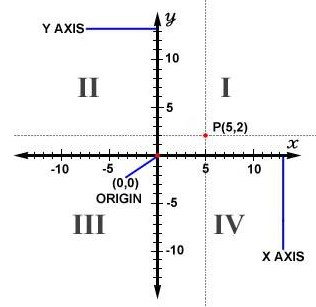
\includegraphics[width=0.9\textwidth]{img/quadrant.jpg}
        \caption*{Source: \href{http://www.csgnetwork.com/coordinatedistancecalc.html}{CSGNetwork}}
      \end{figure}
    \end{columns}
\end{frame}

\begin{frame}[fragile]{Summary Exercise}
  Expected output:
\begin{lstlisting}[language=bash]
  ./main        ./main        ./main        ./main
  1.3 4.5       -1.4 2.0      -3.2 -4.4     3.3 -3.1
  Quadrant 1    Quadrant 2    Quadrant 3    Quadrant 4

  ./main        ./main        ./main        
  0 4.5         -3.3 0        0 0     
  UNDEFINED      UNDEFINED    UNDEFINED
\end{lstlisting}
\end{frame}

\begin{frame}{Summary Exercise}

  \begin{enumerate}
    \setcounter{enumi}{2}
    \item Write a program to find the eligibility of admission for a professional course based on the following criteria:\\
    \vspace{1mm}
    Eligibility Criteria : Marks in Maths >=65 and Marks in Phy >=55 and Marks in Chem>=50 and Total in all three subject >=190 or Total in Maths and Physics >=140 
  \end{enumerate}
\end{frame}

\begin{frame}[fragile]{Summary Exercise}
  Expected output:
  \begin{itemize}
    \item Math = 17, Phy = 32, Chem = 1
\begin{lstlisting}[language=bash]
  ./main
  17 32 1
  Not Eligible
\end{lstlisting}
    \item Math = 70, Phy = 65, Chem = 55
\begin{lstlisting}[language=bash]
  ./main
  70 65 55
  Eligible
\end{lstlisting}
    \item Math = 70, Phy = 69, Chem = 99
\begin{lstlisting}[language=bash]
  ./main
  70 69 99
  Eligible
\end{lstlisting}
  \end{itemize}
\end{frame}

\begin{frame}[fragile]{Summary Exercise}
  \begin{enumerate}
    \setcounter{enumi}{3}
    \item Every year that is exactly divisible by four is a leap year, except for years that are exactly divisible by 100, but these centurial years are leap years if they are exactly divisible by 400. For example, the years 1700, 1800, and 1900 are not leap years, but the years 1600 and 2000 are. Write a program that determines whether a year is a leap year.
  \end{enumerate}
\begin{lstlisting}
  $./main             ./main              ./main
  1700                1600                2012
  Not leap year       Is leap year        Is leap year
\end{lstlisting}
\end{frame}

\begin{frame}{Boolean arithmetic}
  \begin{itemize}
    \item We have just looked at conditional statements that are connected using not, or, and operators
    \item In fact there are algebraic structure associated with these operators called \textbf{boolean arithmetic}
    \item Understanding these arithmetic rules can help us simply and rewrite our conditional statements
  \end{itemize}
\end{frame}

\begin{frame}{Properties of boolean operators}
  \begin{itemize}
    \item Associativity
    \begin{enumerate}
      \item $x\lor (y\lor z) = (x\lor y) \lor z$
      \item $x\land (y\land z) = (x\land y) \land z$
    \end{enumerate}
    \item Commutativity
    \begin{enumerate}
      \item $x\lor y = y \lor x$
      \item $x\land y  = y\land x$
    \end{enumerate}
    \item Distributive of $\land$ over $\lor$
    \begin{enumerate}
      \item $x \land (y\lor z) = (x \land y) \lor (x \land z)$\\
      \item $x \lor (y\land z) = (x\lor y) \land (x\lor z)$
    \end{enumerate}
  \end{itemize}
\end{frame}

\begin{frame}{Properties of boolean operations}
  \begin{itemize}
    \item Identities
    \begin{enumerate}
      \item $x\lor F = x$
      \item $x \land T = x$
    \end{enumerate}
    \item Annihilators
    \begin{enumerate}
      \item $x\lor T = T$
      \item $x\land F = F$
    \end{enumerate}
    \item Double negation
    \begin{enumerate}
      \item $\neg (\neg x) = x $
    \end{enumerate}
    \item De Morgan's law
    \begin{enumerate}
      \item $\neg (x \lor y) = \neg x \land \neg y$
      \item $\neg (x \land y) = \neg x \lor \neg y$
    \end{enumerate}
  \end{itemize}
\end{frame}
\begin{frame}{Exercise}
  Prove the following Identities:
  \begin{enumerate}
    \item $x\land (x\lor y) = x$
    \item $\neg x \land y = \neg (\neg y) \land \neg x$
    \item $a = b \land a$ if and only if $b = a \lor b$
    \item Prove by the De Morgan's law by truth table
    \item Prove by the distributive laws by truth table
    \item Define $x\rightarrow y = \neg x \land y$. Show that $(x \land y) \rightarrow y = T$
    \item Define $x \leftrightarrow y = (x \rightarrow y) \land (y \rightarrow x)$. Show that $x\leftrightarrow y = (x\land y)\lor (\neg x \land \neg y)$ 
    \item Simplify$(x \lor y) \land \neg (\neg x \land y)$ 
  \end{enumerate}
\end{frame}

\begin{frame}{Mathematical proving}
  \begin{itemize}
    \item A \textbf{mathematical proof} is a sequence of logical statements, one implying another, which gives an explanation of why a given statement is true. 
    \item Mathematical proof is \textit{absolute}, which means that once a theorem is proved, it is proved for ever.
  \end{itemize}  
\end{frame}

\begin{frame}{Mathematical proving}
  \begin{exampleblock}{Example: Geometric sequence}
    One day, Judy is bored. So she tries to play around with sum of power of two. She tabulated her some an found out something interesting: 
    \begin{table}[]
      \begin{tabular}{lll}
      1 & $2^1 = 2$  & $1+2 = 3$                            \\
      2 & $2^2 = 4$  & $1+2+ 2^2 = 7$                       \\
      3 & $2^3 = 8$  & $1+2+2^2 + 2^3 = 15$                 \\
      4 & $2^4 = 16$ & $1 + 2 + 2^2 + 2^3 + 2^4 = 31$       \\
      5 & $2^5 = 32$ & $1 + 2 + 2^2 + 2^3 + 2^4 + 2^5 = 63$
      \end{tabular}
      \end{table}
  \end{exampleblock}
\end{frame}

\begin{frame}{Mathematical proving}
  So she made the following hypothesis:
  \begin{block}{Hypothesis}
    Let $n$ be an integer and $n\geq 1$. Then $1+2+\cdots + 2^{n-1} = 2^n -1$\\
    \textbf{\textit{Question: Is she correct? }}
  \end{block}
\end{frame}

\begin{frame}{Mathematical proving}
  In fact she IS correct. To see that, let $S$ be the required sum:
  \begin{align*}
    S = 1 + 2 + 2^2 + \cdots + 2^{n-2} + 2^{n-1}
  \end{align*}
  Then $2S$ is:
  \begin{align*}
    2S = 2 + 2^2 + 2^3 + \cdots + 2^{n-1} + 2^{n}
  \end{align*}
\end{frame}

\begin{frame}{Mathematical proving}
  So:
  \begin{align*}
    S &= 2S - S\\
    &= (2 + 2^2 + 2^3 + \cdots + 2^{n-1} + 2^{n}) - (1 + 2 + 2^2 + \cdots + 2^{n-2} + 2^{n-1})\\
    &= 2^n - 1
  \end{align*}
  Which proves our hypothesis. Now, even if we don't list out every single number $n$, we will know the claim is true.
\end{frame}

\begin{frame}{Mathematical proving}
  \begin{itemize}
    \item This is an example of a proof
    \item In general, we need a proof in order to be certain something is true, because apparent patterns can and had failed in the past 
    \item Example:
    \item \textbf{Claim:} $n^2 + n + 41$ is a prime number (which is false)
  \end{itemize}  
  \begin{table}[]
    \begin{tabular}{lllllllll}
    $n$        & 1   & 2   & 3   & 4   & $\cdots$ & 38   & 39   & 40   \\
    $n^2+n+41$ & 43  & 47  & 53  & 61  & $\cdots$ & 1523 & 1601 & 1681 \\
    Is prime?  & Yes & Yes & Yes & Yes & $\cdots$ & Yes  & Yes  & No  
    \end{tabular}
    \end{table}
\end{frame}

\begin{frame}{Mathematical proving}
  \begin{exampleblock}{Exercise}
    \begin{itemize}
      \item Prove that $n(n+1)$ is always divisble by 2
      \item In a group of $366$ people, there must be at least two people with the same birthday
      \item Prove that is impossible to write $\sqrt{2} = \frac{m}{n}$ where $m,n$ are integers
      \item Let $x$ be a real number and $0<x<1$. Show that if $n$ is the smallest positive integer such that $x-1/n \geq 0$, then $x-1/n < 1/n$
    \end{itemize}
  \end{exampleblock}
\end{frame}

\begin{frame}{(Optional) Proof by contrapositive}
  \begin{itemize}
    \item The result provide the grounding for a method of proof called \textbf{proof by contrapositive}
    \item In short, because $p \rightarrow q$ is equivalent to $\neg q \rightarrow \neg p$, we can prove a statement by it's contrapositive, which is sometimes easier
    \item Consider the following claim:
    \item \textbf{Claim:}
      Let $x\in\mathbb{Z}^+$. If $x^2 -6x + 5$ is even, then $x$ is odd.
    \item How can we prove this claim?
  \end{itemize}
\end{frame}
\begin{frame}{(Optional) Proof by contrapositive}
  \begin{itemize}
    \item Instead proving directly, we prove it's contrapositive. 
    \item The contrapositive of the statement is:
    \item \textbf{Contrapositive Claim:} If $x$ is even, then $x^2 - 6x + 5$ is odd
    \item This is almost trivial to prove, because:
    \begin{align*}
      x^2 - 6x + 5 = \overbrace{x(x-6)}^{\text{even if x even}} + \overbrace{5}^{\text{odd}}
    \end{align*}
    So the sum must be odd
  \end{itemize}
\end{frame}


\begin{frame}{Boolean arithmetic}
  \begin{itemize}
    \item We have just looked at conditional statements that are connected using not, or, and operators
    \item In fact there are algebraic structure associated with these operators called \textbf{boolean arithmetic}
    \item Understanding these arithmetic rules can help us simply and rewrite our conditional statements
  \end{itemize}
\end{frame}

\begin{frame}{Properties of boolean operators}
  \begin{itemize}
    \item Associativity
    \begin{enumerate}
      \item $x\lor (y\lor z) = (x\lor y) \lor z$
      \item $x\land (y\land z) = (x\land y) \land z$
    \end{enumerate}
    \item Commutativity
    \begin{enumerate}
      \item $x\lor y = y \lor x$
      \item $x\land y  = y\land x$
    \end{enumerate}
    \item Distributive of $\land$ over $\lor$
    \begin{enumerate}
      \item $x \land (y\lor z) = (x \land y) \lor (x \land z)$\\
      \item $x \lor (y\land z) = (x\lor y) \land (x\lor z)$
    \end{enumerate}
  \end{itemize}
\end{frame}

\begin{frame}{Properties of boolean operations}
  \begin{itemize}
    \item Identities
    \begin{enumerate}
      \item $x\lor F = x$
      \item $x \land T = x$
    \end{enumerate}
    \item Annihilators
    \begin{enumerate}
      \item $x\lor T = T$
      \item $x\land F = F$
    \end{enumerate}
    \item Double negation
    \begin{enumerate}
      \item $\neg (\neg x) = x $
    \end{enumerate}
    \item De Morgan's law
    \begin{enumerate}
      \item $\neg (x \lor y) = \neg x \land \neg y$
      \item $\neg (x \land y) = \neg x \lor \neg y$
    \end{enumerate}
  \end{itemize}
\end{frame}
\begin{frame}{Exercise}
  Prove the following Identities:
  \begin{enumerate}
    \item $x\land (x\lor y) = x$
    \item $\neg x \land y = \neg (\neg y) \land \neg x$
    \item $a = b \land a$ if and only if $b = a \lor b$
    \item Prove by the De Morgan's law by truth table
    \item Prove by the distributive laws by truth table
    \item Define $x\rightarrow y = \neg x \land y$. Show that $(x \land y) \rightarrow y = T$
    \item Define $x \leftrightarrow y = (x \rightarrow y) \land (y \rightarrow x)$. Show that $x\leftrightarrow y = (x\land y)\lor (\neg x \land \neg y)$ 
    \item Simplify$(x \lor y) \land \neg (\neg x \land y)$ 
  \end{enumerate}
\end{frame}

\end{document}
